\chapter{Dise�o de la integraci�n}

Este es un cap�tulo que tiene como objetivo explicar como se integran entre si las herramientas del proyecto, Ksensor con las modificaciones expuestas y los m�dulos de trazas y estad�sticas. Para guiar la explicaci�n, se puede referir a  \reference{fig:integracion-modular}{Figura de integraci�n de los m�dulos}

\begin{figure}[h]
\centering
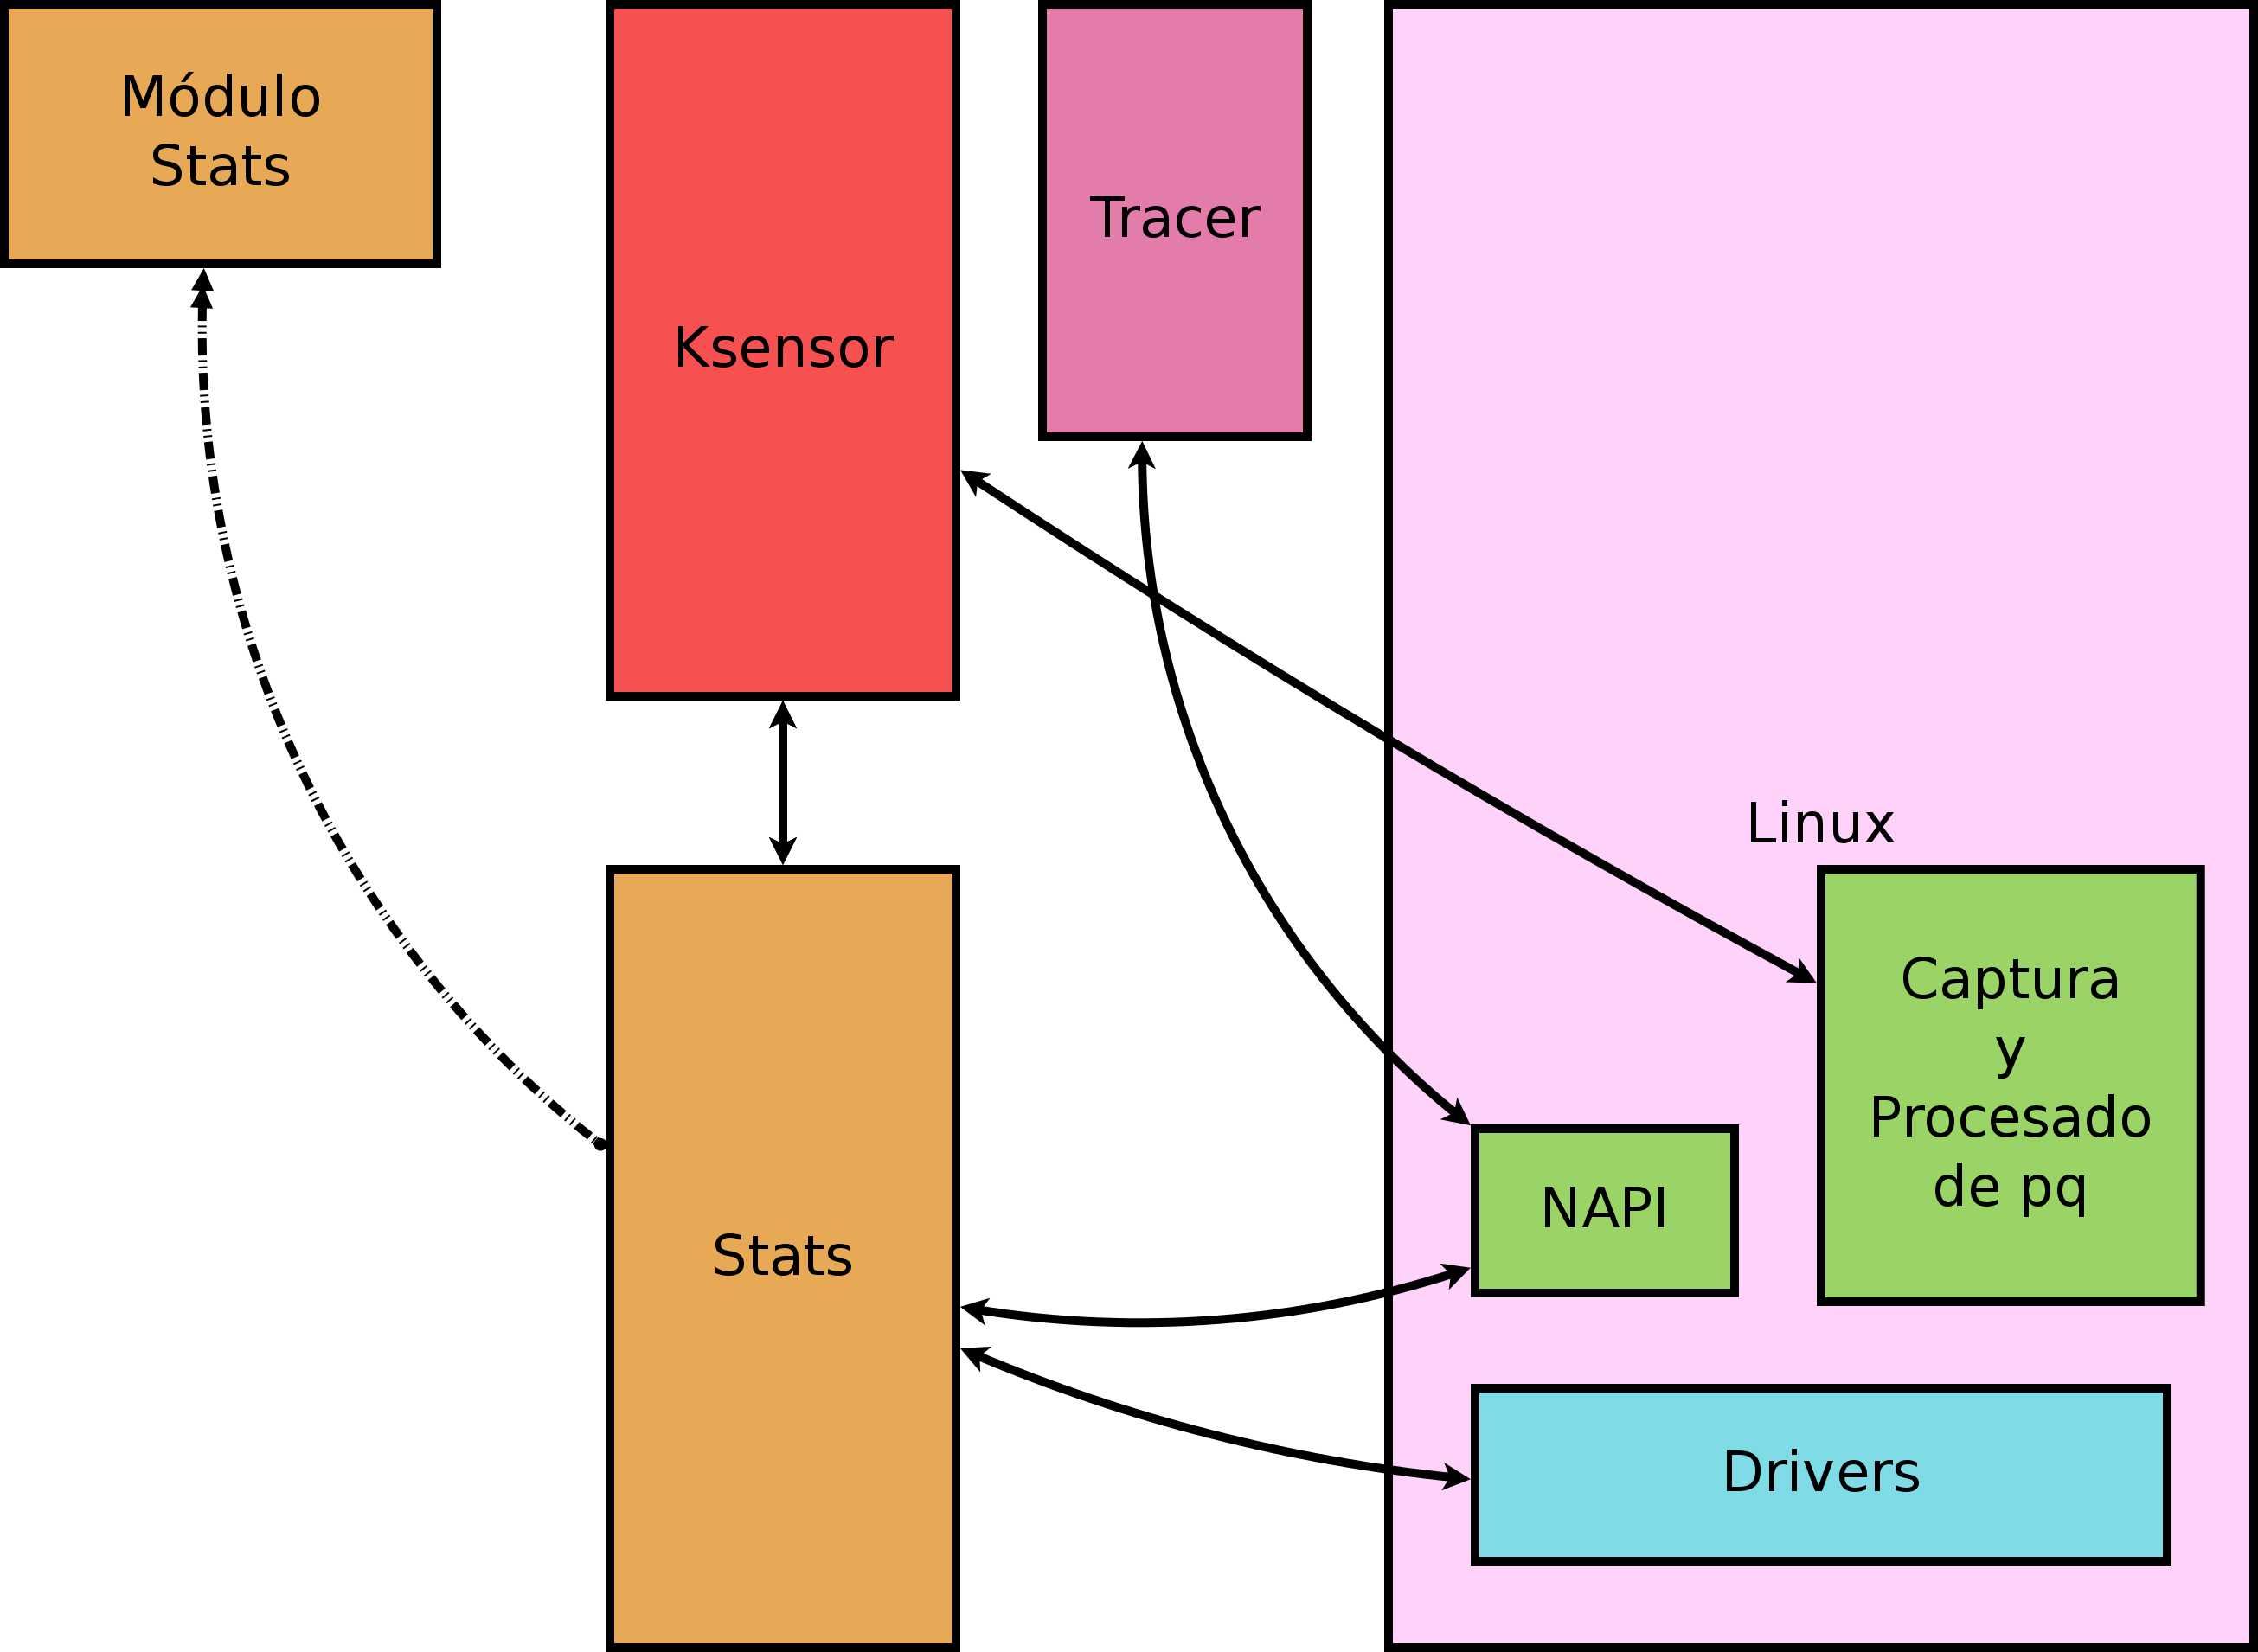
\includegraphics[width=\linewidth]{Integracion}
\caption{Integraci�n de los m�dulos entre si}
\label{fig:integracion-modular}
\end{figure}

En la figura, se han referenciado las 3 partes que componen el kernel, y donde se introduce o modifica c�digo. Apoyando la explicaci�n en la figura, se explicar� la integraci�n entre ksensor y los m�dulos.

\section{Ksensor y el m�dulo de estad�sticas}

En la figura se ha representado el m�dulo de estad�sticas como un m�dulo compuesto de dos partes, una propiamente dicha, el m�dulo, la parte que se puede insertar y extraer, y la parte que est� est�ticamente integrada en el kernel.

Dependiendo de las opciones de compilaci�n, en caso de habilitar Ksensor y el m�dulo de estad�sticas simult�neamente, se activan directamente las estad�sticas dentro de Ksensor, a parte de las estad�sticas internas del mismo. En caso de no habilitar Ksensor, el m�dulo de estad�sticas se compilar�a con solo una parte de las mismas.

\section{Ksensor y el m�dulo de trazas}

Este m�dulo ha sido dise�ado para tener un funcionamiento al margen de Ksensor, y de hecho en la implementaci�n actual, tracea softirqs, por lo que no se perder�a funcionalidad en este. En caso de implementar trazas dentro de Ksensor, se dejar�an de compilar, pero este m�dulo quedar�a disponible para el resto del sistema.

\section{Estad�sticas y trazas}

Entre estos dos m�dulos, al requerir en algunas partes de c�digo efectuar las mismas medidas, solo interact�an a nivel de implementaci�n. En el dise�o de bajo nivel se dar�n explicar� de una forma m�s concreta el tipo de interacci�n que tienen.